%%%%%%%%%%%%%%%%%%%%%%%%%%%%%%%%%%%%%%%%%
% Beamer Presentation
% LaTeX Template
% Version 1.0 (10/11/12)
%
% This template has been downloaded from:
% http://www.LaTeXTemplates.com
%
% License:
% CC BY-NC-SA 3.0 (http://creativecommons.org/licenses/by-nc-sa/3.0/)
%
%%%%%%%%%%%%%%%%%%%%%%%%%%%%%%%%%%%%%%%%%

%----------------------------------------------------------------------------------------
%	PACKAGES AND THEMES
%----------------------------------------------------------------------------------------

\documentclass{beamer}

\mode<presentation> {

% The Beamer class comes with a number of default slide themes
% which change the colors and layouts of slides. Below this is a list
% of all the themes, uncomment each in turn to see what they look like.

%\usetheme{default}
%\usetheme{AnnArbor}
%\usetheme{Antibes}
%\usetheme{Bergen}
%\usetheme{Berkeley}
%\usetheme{Berlin}
%\usetheme{Boadilla}
%\usetheme{CambridgeUS}
%\usetheme{Copenhagen}
%\usetheme{Darmstadt}
%\usetheme{Dresden}
%\usetheme{Frankfurt}
%\usetheme{Goettingen}
%\usetheme{Hannover}
%\usetheme{Ilmenau}
%\usetheme{JuanLesPins}
%\usetheme{Luebeck}
\usetheme{Madrid}
%\usetheme{Malmoe}
%\usetheme{Marburg}
%\usetheme{Montpellier}
%\usetheme{PaloAlto}
%\usetheme{Pittsburgh}
%\usetheme{Rochester}
%\usetheme{Singapore}
%\usetheme{Szeged}
%\usetheme{Warsaw}

% As well as themes, the Beamer class has a number of color themes
% for any slide theme. Uncomment each of these in turn to see how it
% changes the colors of your current slide theme.

%\usecolortheme{albatross}
%\usecolortheme{beaver}
%\usecolortheme{beetle}
%\usecolortheme{crane}
%\usecolortheme{dolphin}
%\usecolortheme{dove}
%\usecolortheme{fly}
%\usecolortheme{lily}
%\usecolortheme{orchid}
%\usecolortheme{rose}
%\usecolortheme{seagull}
%\usecolortheme{seahorse}
%\usecolortheme{whale}
%\usecolortheme{wolverine}

%\setbeamertemplate{footline} % To remove the footer line in all slides uncomment this line
%\setbeamertemplate{footline}[page number] % To replace the footer line in all slides with a simple slide count uncomment this line

%\setbeamertemplate{navigation symbols}{} % To remove the navigation symbols from the bottom of all slides uncomment this line
}

\usepackage{graphicx} % Allows including images
\usepackage{booktabs} % Allows the use of \toprule, \midrule and \bottomrule in tables

%----------------------------------------------------------------------------------------
%	TITLE PAGE
%----------------------------------------------------------------------------------------

\title[social and financial interactions]{Interplay between social and financial interactions in a crypto-currency } % The short title appears at the bottom of every slide, the full title is only on the title page

\author{\textbf{Nicolas Gensollen}, Matthieu Latapy} % Your name
\institute[LIP6] % Your institution as it will appear on the bottom of every slide, may be shorthand to save space
{
Laboratoire d'informatique de Paris 6 \\ % Your institution for the title page
\medskip
\textit{nicolas.gensollen@lip6.fr} % Your email address
}
\date{\today} % Date, can be changed to a custom date

\begin{document}

\begin{frame}
\titlepage % Print the title page as the first slide
\end{frame}

\begin{frame}
\frametitle{Overview} % Table of contents slide, comment this block out to remove it
\tableofcontents % Throughout your presentation, if you choose to use \section{} and \subsection{} commands, these will automatically be printed on this slide as an overview of your presentation
\end{frame}

%----------------------------------------------------------------------------------------
%	PRESENTATION SLIDES
%----------------------------------------------------------------------------------------



%------------------------------------------------
\section{Context} 
%------------------------------------------------

\begin{frame}
\Huge{\centerline{Context}}
\end{frame}


%------------------------------------------------
\subsection{Who are we?}
%------------------------------------------------

\begin{frame}
	\frametitle{Who we are and what we do}
	\textbf{Our team}
	\begin{itemize}
		\item Complex Networks team (LIP6).
		\item Internet measurements, random graphs, temporal networks
		\item Social network analysis, spreading phenomena, graph algorithms
	\end{itemize}
	\bigskip
	\textbf{Our main research topics}
	\bigskip
	\begin{columns}[t]
		\column{.4\textwidth} % Left column and width
		\textbf{Stream Graphs}
		\begin{figure}
			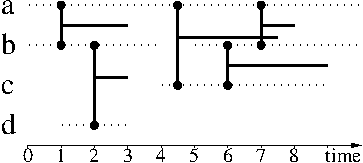
\includegraphics[width=0.8\linewidth]{./figures/stream_graph}
		\end{figure}
		\column{.6\textwidth} % Right column and width
		\textbf{Anomaly detection}
		\begin{figure}
			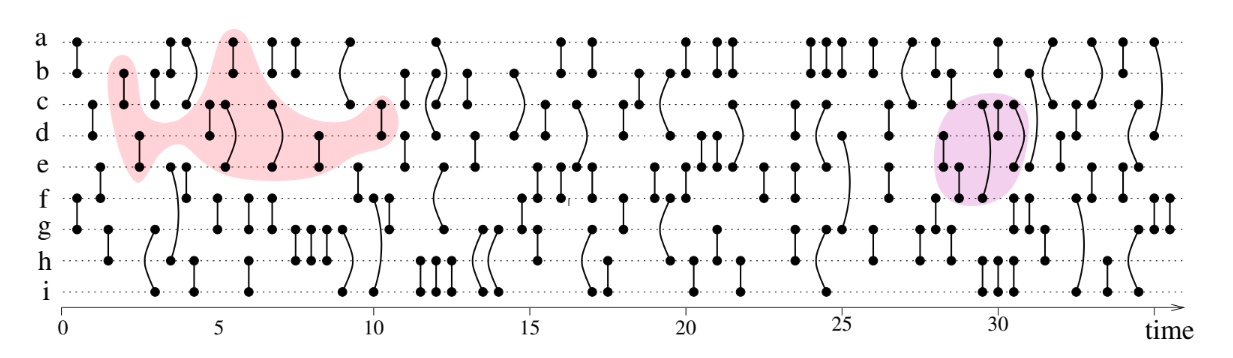
\includegraphics[width=\linewidth]{./figures/anomalie_detection}
		\end{figure}
	\end{columns}
\end{frame}


%------------------------------------------------
\subsection{The G1 crypto-currency}
%------------------------------------------------

\begin{frame}
	\frametitle{The G1 crypto-currency}
	\begin{columns}[c]
		\column{.7\textwidth}
		\begin{itemize}
			\item Created in 2017 in France
			\item \textbf{Particularity:} first "\textit{libre}" crypto-currency
			\item \textbf{Spatial} and \textbf{Temporal} symmetry principles
		\end{itemize}
		\column{.3\textwidth}
		\begin{figure}
			
\includegraphics[width=.5\linewidth]{./figures/g1_logo}
		\end{figure}
	\end{columns}
	\bigskip
	\begin{itemize}
		\item \textbf{Monetary creation} is \textbf{automatic} and \textbf{divided equally} among the members\footnote{Relative Theory of Money, \textit{https://en.trm.creationmonetaire.info/}}
		\item Each member receives one \textit{Universal Dividend} every day
	\end{itemize}
\end{frame}

%------------------------------------------------

\begin{frame}
	\frametitle{The G1 crypto-currency}
	\begin{figure}
		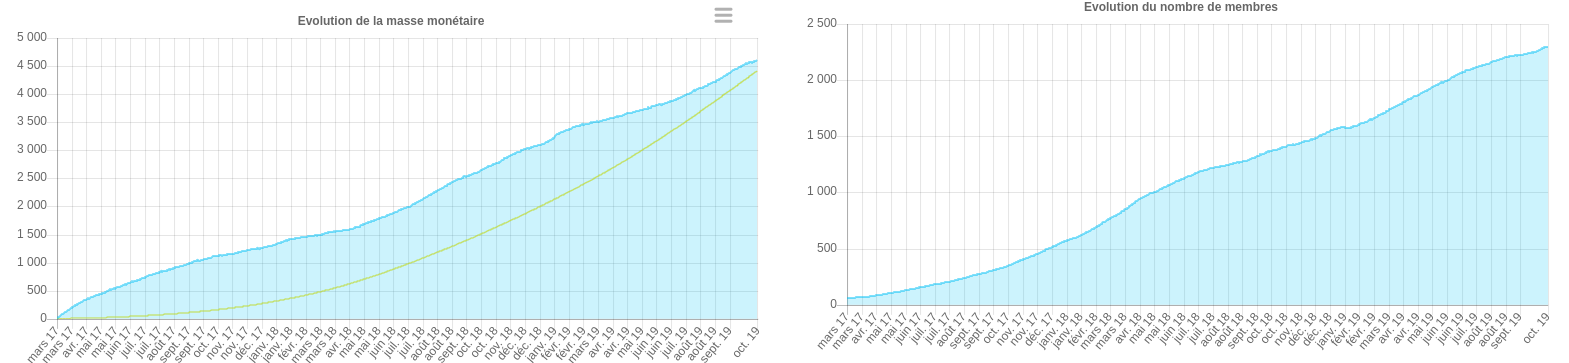
\includegraphics[width=\linewidth]{./figures/g1_evolution}
		\caption{\textbf{Left -} Evolution of the monetary mass. \textbf{Right -} Evolution of the number of members. Source: Cesium client (\textit{https://g1.duniter.fr/\#/app/currency/lg})}
	\end{figure}
	\smallskip
	\textbf{Some numbers (Oct. 2019)}
	\begin{columns}[c]
		\column{.5\textwidth}
		\begin{itemize}
			\item About 2300 identified members.
			\item $UD \simeq 10\ \tilde{G}1\ /\ day$ .
		\end{itemize}
		\column{.5\textwidth}
		\begin{itemize}
			\item Monetary growth: $0.22\%\ /\ day$.
			\item Monetary mass per member: $4600 \tilde{G}1 $.
		\end{itemize}
	\end{columns}
\end{frame}

%------------------------------------------------

\begin{frame}
	\frametitle{The G1 crypto-currency}
	\begin{columns}[c]
		\column{.5\textwidth}
		\begin{itemize}
			\item Identities of members are a key concern!
			\item \textbf{1 member = 1 real living human being}
			\item Members are identified through a \textit{Web of Trust} (WoT) mechanism
		\end{itemize}
		\column{.5\textwidth}
		\begin{figure}
			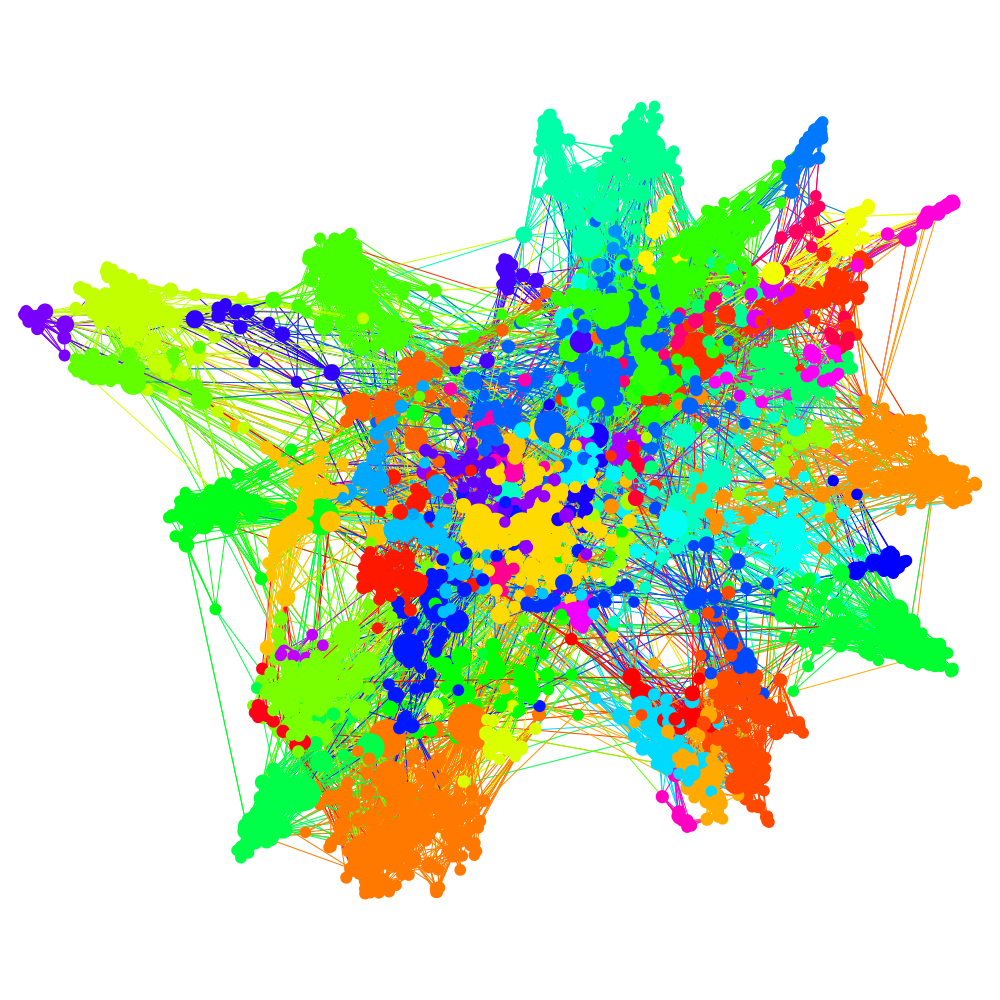
\includegraphics[width=.7\linewidth]{./figures/wot}
		\end{figure}
	\end{columns}
	\begin{itemize}
		\item Member accounts are different from regular accounts.
		\item Safety rules are constraining its growth
		\item Examples:
		\begin{itemize}
			\item A new member has to receive at least 5 certifications
			\item All members should be close enough to 				\textit{sentinel members}
		\end{itemize}
	\end{itemize}
\end{frame}


%------------------------------------------------
\subsection{Objectives of this work}
%------------------------------------------------

\begin{frame}
	\frametitle{Objectives of this work}
	\begin{itemize}
		\item We can extract from the blockchain a stream of transactions $\mathcal{T}$ and a stream of certifications $\mathcal{C}$.
		\item A transaction $\left(t,u,v,a\right) \in \mathcal{T}$: \textit{Entity $u$ sends amount $a$ to entity $v$ at time $t$}.
		\item A certification $\left(t,u,v\right) \in \mathcal{C}$: \textit{Member $u$ certifies the identity of members $v$ at time $t$}.
		\item We have a dynamic network of social ties and financial transactions between identified human beings!
	\end{itemize}
	\medskip
	\textbf{Unique dataset to study the interplay between money exchange and social ties.}
\end{frame}



%------------------------------------------------
\section{Approach and basic results}
%------------------------------------------------

\begin{frame}
	\Huge{\centerline{Approach and basic results}}
\end{frame}


%------------------------------------------------
\subsection{Approach}
%------------------------------------------------

\begin{frame}
	\frametitle{Approach}
	\begin{figure}
		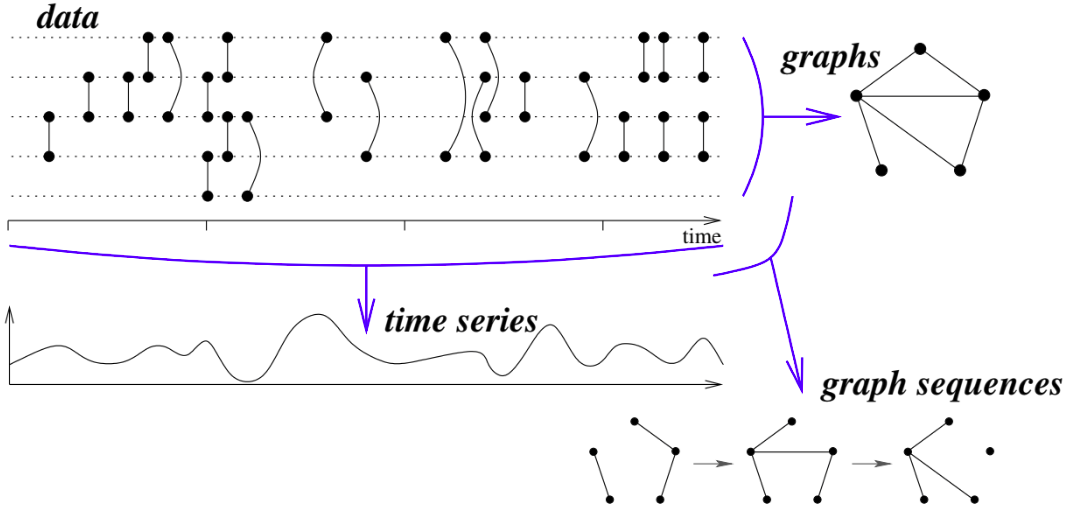
\includegraphics[width=.8\linewidth]{./figures/stream_graph_signal}
	\end{figure}
	\begin{itemize}
		\item The data is best modeled by stream graphs
		\item Start with simpler models (timeseries and graphs) to gain insight
		\item Then use stream graphs to capture more complex dependencies
	\end{itemize}
\end{frame}


%------------------------------------------------
\subsection{Basic Results}
%------------------------------------------------

\begin{frame}
	\frametitle{Activity}
	\begin{block}{Activity of a stream}
We can define the \textit{activity} of a stream $S$ as the time serie of the number of links.
	\end{block}
	\bigskip
	\begin{figure}
		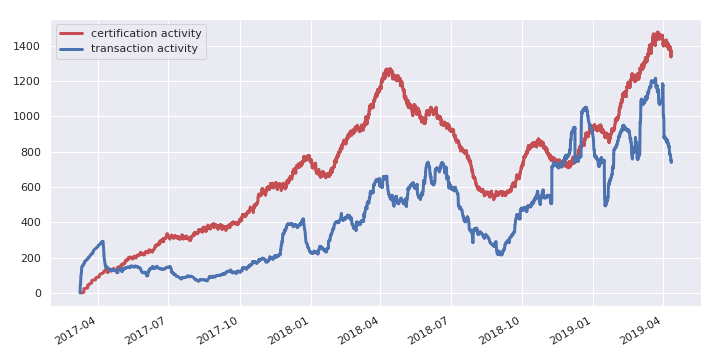
\includegraphics[width=.8\linewidth]{./figures/activity}
		\caption{30 days rolling sum of the activities of $ \mathcal{C}$ (red curve) and $\mathcal{T}$ (blue curve).}
	\end{figure}
\end{frame}

%------------------------------------------------

\begin{frame}
	\frametitle{Induced Graphs}
	\begin{block}{Graph induced by a stream}
	The graph induced by a stream $S = \left(T, V, W, E \right)$ is a static graph $ G \left(S \right) = \left(V, \bar{E} \right)$ in which two nodes are linked if they interacted at least once in the stream, i.e. $ \bar{E} = \left\{ \left( u, v \right),\ \exists \left(t, uv \right) \in E \right\}$.
	\end{block}
	\bigskip
	\begin{figure}
		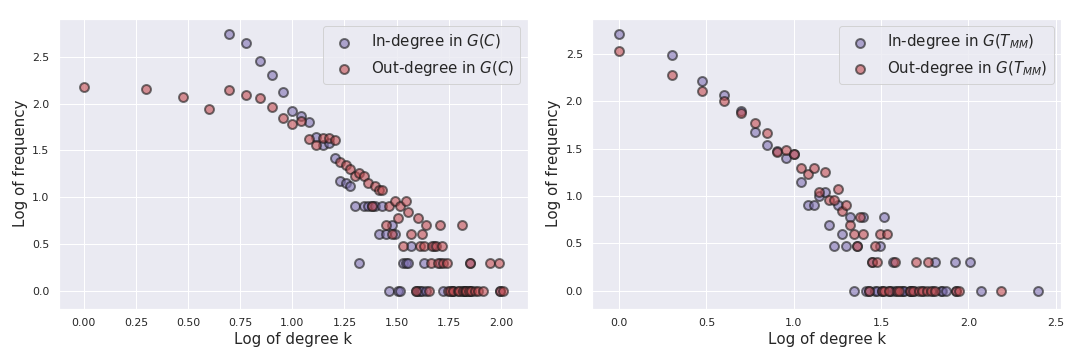
\includegraphics[width=.9\linewidth]{./figures/degree_distribution}
		\caption{\textbf{Left -} In-degree (in blue) and out-degree (in red) distributions of $G \left( \mathcal{C} \right)$. \textbf{Right -} In-degree (in blue) and out-degree (in red) distributions of $G \left( \mathcal{T} \right)$.}
	\end{figure}
\end{frame}



%------------------------------------------------
\section{Certifications and Transactions}
%------------------------------------------------

\begin{frame}
	\Huge{\centerline{Certifications and Transactions}}
\end{frame}

%------------------------------------------------

\begin{frame}
	\frametitle{Time between certifications and transactions}
	\begin{figure}
		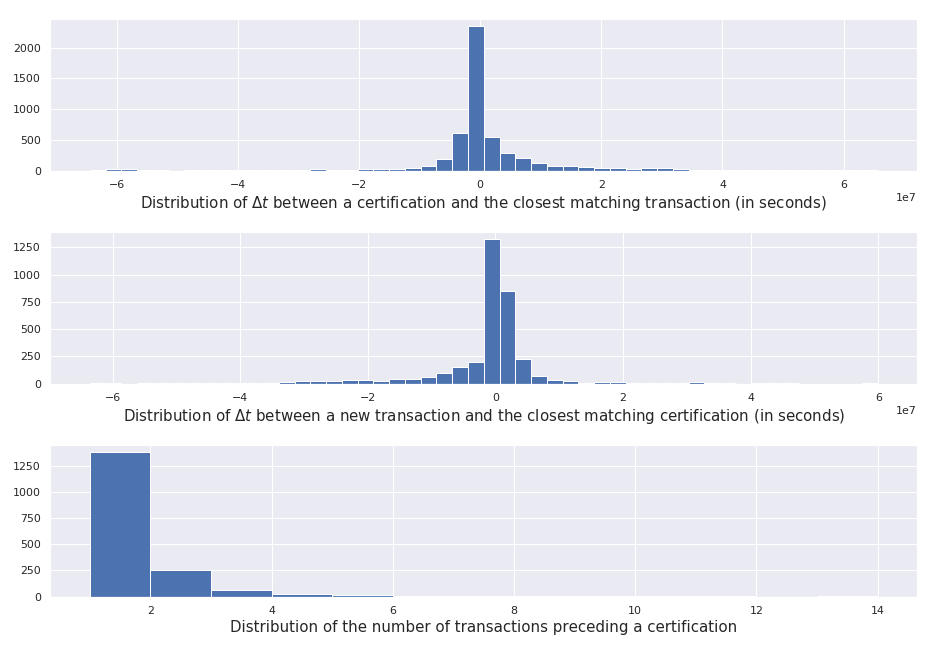
\includegraphics[width=.9\linewidth]{./figures/delta_t}
	\end{figure}
\end{frame}

%------------------------------------------------

\begin{frame}
	\frametitle{K-Closures}
	\begin{figure}
		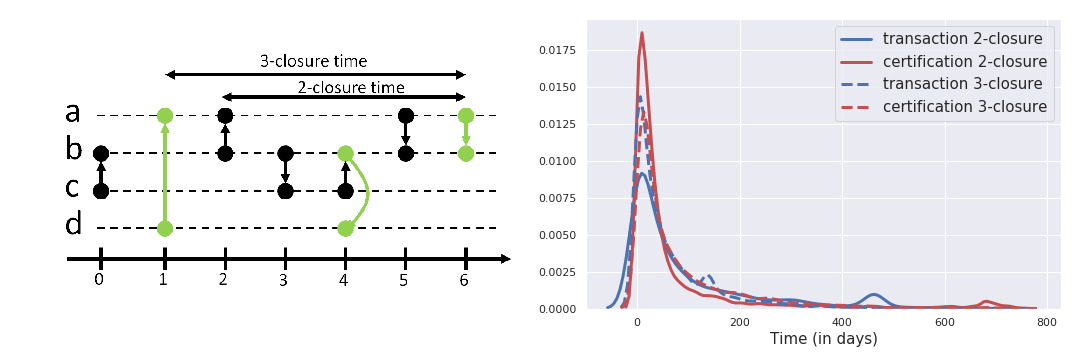
\includegraphics[width=\linewidth]{./figures/triadic_closure}
		\caption{\textbf{Left -} Schematic view of the 2 and 3-closures. The 2-closure of link $\left(6, ab \right)$ is equal to 4 since we have to go back to $t = 2$ to find a reversed link (e.g. $\left(2, ba \right)$). The 3-closure of link $\left(6, ab \right)$ is equal to 5 since we have to go back to $t = 1$ to close the triangle composed of $\left(6, ab\right)$, $\left(4, bd \right)$, $\left(1, da\right)$. \textbf{Right -} The densities of 2 and 3-closures for all links in $\mathcal{C}$ and $\mathcal{T}$.}
	\end{figure}
\end{frame}


%------------------------------------------------

\begin{frame}
	\Huge{\centerline{The End}}
\end{frame}

%----------------------------------------------------------------------------------------

\end{document} 